\chapter{Gathering data from +CityxChange} 
\label{chap:survey}

This section introduces a survey conducted to understand the the needs of the +CityxChange \gls{eaf}.

\section{Motivation behind the survey}
A survey was found to be the best approach to understanding the role of \gls{ea} in smart city projects and how it relates to learning. +CityxChange was chosen as a project where the survey could be undertaken. As an ongoing lighthouse project involving two lighthouse cities and five follower cities, it is believed to be representative of smart city projects.
The main motivation of the survey was to gain insights from the +CityxChange employees that had used the +CityxChange \gls{eaf}. Their understanding could be used to improve \gls{ea} in regards to learning in smart city projects. The survey was made to understand the context where the \gls{ea} was used, who were using it, what their attitudes towards it were and what could be done to improve it. The secondary motivation was for this information to be used to improve the +CityxChange \gls{eaf} to support learning across cities.
The full questionnaire can be found in apendix \ref{app:questionnaire}.

\section{Survey Results}
\subsection{Demographic}
The demographics section asked for gender, age represented organisation and role within organisation.
Overall the demographic information is inline with what was expected in the field of \gls{ea} and computer science. 
The roles reported varied, but could be summed up as researchers, developers, engineers and managerial roles.
\begin{figure}
    \centering
    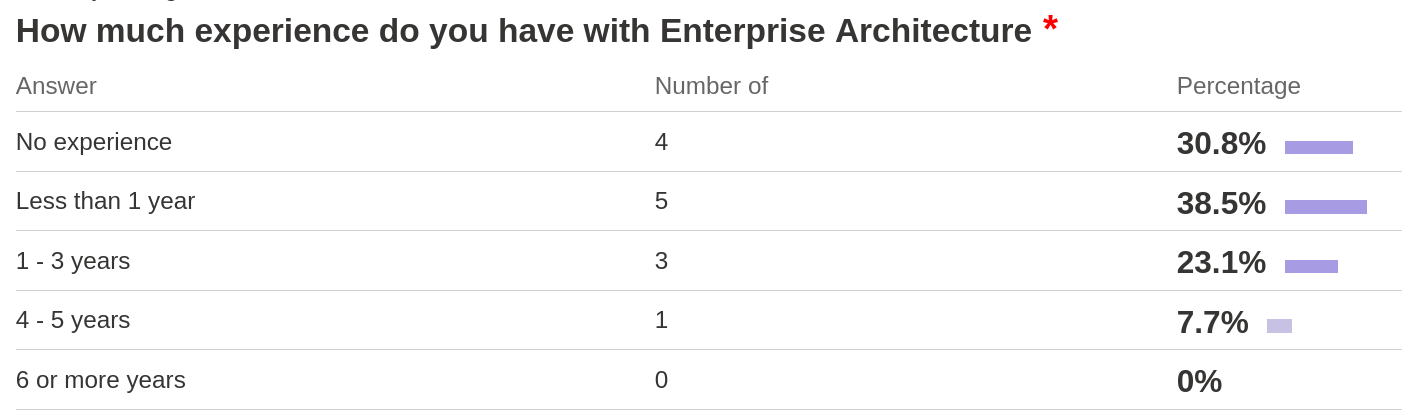
\includegraphics[scale=0.35]{figures/png/questionnaire_EA_Experience.png}
    \caption{Questionnaire demographic on EA experience}
    \label{fig:questionnaire-ea-experience}
\end{figure}

\begin{figure}
    \centering
    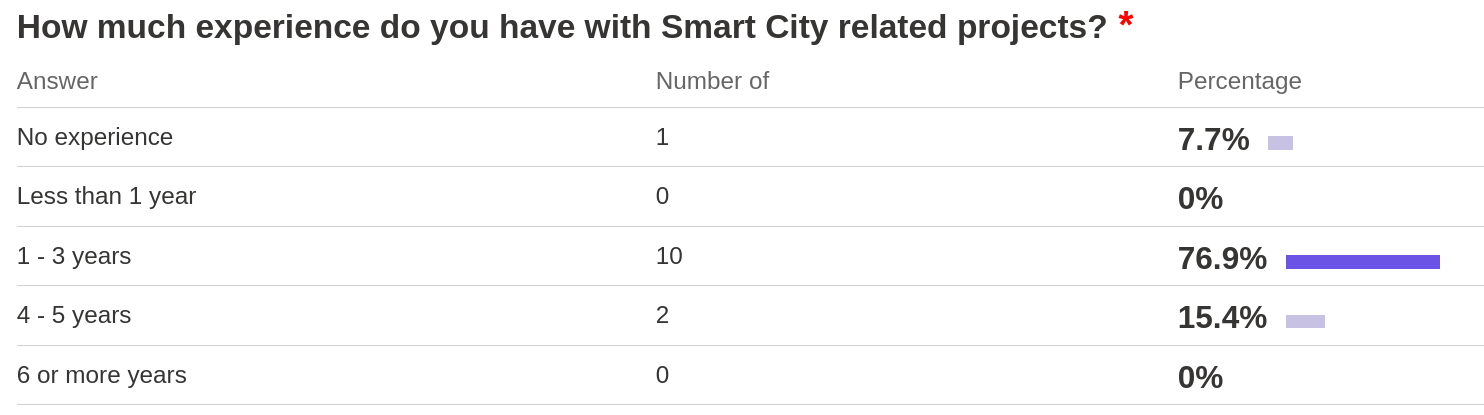
\includegraphics[scale=0.33]{figures/png/questionnaire_SmartCity_Experience.png}
    \caption{Questionnaire demographic on smart city experience}
    \label{fig:questionnaire-smartcity-experience}
\end{figure}



Figure \ref{fig:questionnaire-ea-experience} and \ref{fig:questionnaire-smartcity-experience} show the participants experience with \gls{ea} and smart city projects respectively. It shows that a significant percentage of participants have little experience with \gls{ea}. This makes it hard to trust some of the data in regards to quality of the \gls{eaf} and \gls{ea} model, but also shows the level of expertise of the users. It is clear that the models must be understood by those with little experience with \gls{ea}. The participants had more experience with smart city projects. This makes the domain specific questions more trustworthy. 

\subsection{Ease of use and usefulness}
The questionnaire results indicate that \gls{ea} in general and the +CityxChange \gls{eaf} in particular are seen as useful in the +CityxChange project, but the \gls{eaf} is not easy to understand. 

\subsection{How it relates to knowledge transfer}
The questionnaire results indicate that the \gls{eaf} could be useful for both retaining and sharing knowledge.

\subsection{Free-text answers}
Due to the nature of these questions, no statistical analysis was conducted. It is still seen that valuable information could be drawn from them. The answers indicate that the organisations vary greatly in how they approach knowledge retention and transfer and all of them use multiple approaches. The methods used include both formal and informal methods. Only one answer indicated that their organisation was considering changes or additional methods to retain or transfer knowledge within their organisation. This could indicate that most find their current methods satisfactory. 

Most answers indicated that their organisation did not use any other \gls{ea} approaches than the +CityxChange \gls{eaf}. One answer mentioned using \gls{togaf} while another mentioned an intention to use in the future, but that it was not relevant for +CityxChange. This could indicate that the +CityxChange \gls{eaf} covers its domain well and that modifying the \gls{eaf} for hybrid approaches is not of high importance.

The answers indicated that it was difficult to use without a background in \gls{ea} and that additional value could be gained from lowering the difficulty to a point were non practitioners could understand it. This could indicate that either the detail is too high, that the presentation is difficult to understand or the inherent complexity is problematic. The terminology used in the \gls{eaf} should be reconsidered or clarified.

The last specific question of the questionnaire was in regards to which problems the individual thought should be solved by \gls{ea}. The answers varied a lot with no discernible pattern. It is believed that the question was too broad, but the answers still brought forth a few sentiments that should be considered. A compilation of the answers would be; frameworks and tools for defining and implementing software architecture, aspects of data, regulatory compliance, knowledge retention, digital transformation, \gls{ict} system replication, high level view, cross organisational cooperation, complex systems and sharing of architectural knowledge.

\section{Extracted EA Requirements}
based on the questionnaire and literature, a few requirements were made for the \gls{eaf} and resulting \gls{ea} models.

\begin{itemize}
    \item The \gls{eaf} must be understandable based on the architecture alone for non technical personnel.
    \item The \gls{ea} models must be easy to understand for people with some experience with the \gls{eaf} without thorough understanding of the scenario it describes.
    \item The \gls{eaf} model must be improved with common knowledge retention, sharing and transfer activities in mind.
    \item The \gls{eaf} model must be improved with supplementary technologies in mind. 
    \item Describe which views could be useful for different supplementary activities.
\end{itemize}
